%%%%%%%%%%%%%%%%%%%%%%%%%%
%                          %
% ----- INTRODUCTION ----- %
%                          %
%%%%%%%%%%%%%%%%%%%%%%%%%%

\section{Fonctionnalités}

	La première itération de l'application vise à couvrir certaines des exigences fonctionnelles demandées :
	\begin{itemize}
		\item Fenêtre avec liens dirigeant vers les pages
		\item Page "Cases" affichant la liste des cas avec possibilité d'afficher/cacher des colonnes, et de filtrer des lignes
		\item Page "Patients" affichant la liste des patients avec possibilité d'afficher/cacher des colonnes, et de filtrer des lignes
	\end{itemize}

\section{Conception}

	Le premier prototype de l'application a défini beaucoup des comportements et des mécaniques d'interaction de l'application.

	\subsection{Architecture générale de l'application}

		Tout d'abord, il était nécessaire de réfléchir à l'architecture générale de l'application avant de s'attaquer à chaque partie. Au vu du produit demandé, l'application sera réalisée suivra une architecture classique du schéma Client - Serveur. Du code se trouvera donc exécuté sur le client, et sur le serveur.

	\subsubsection{Frontend}

		La partie frontend est développée à l'aide de React. Il s'agit d'une one-page app : Cela signifie que l'utilisateur utilisera toujours la même adresse web pour accéder à l'application : Celle-ci se chargera ensuite elle-même de se transformer en les diverses interfaces que l'utilisateur va demander.

		Cette page est développée à l'aide de React et de librairies permettant de compléter React, et la structure du code suivra une architecture adaptée à l'utilisation de Flux, dont nous avons parlé précédemment. Il s'agit de l'architecture qu'il est recommandé d'utiliser avec React pour une application de taille moyenne, ce qui correspond à notre projet.

	\subsubsection{Backend}

		La partie backend se compose d'une couche applicative ainsi que d'une base de données. Le client ayant déjà crée une base de données de type MySQL avant le début du projet, elle ne sera pas changée.

		La partie applicative du backend est développée en node.js. Ce choix s'est fait pour des raisons de simplicité : Etant donné que la partie frontend du projet est développée à l'aide d'outils adaptés pour JavaScript, il est assez naturel de continuer le développement du backend avec des technologies similaires.

		La partie base de données restera donc avec MySQL. Quelques changements à la structure de la base de données seront apportés afin que celle-ci soit totalement compatible avec l'application demandée.

	\subsection{Structure de la navigation}

		En plus de répondre aux demandes du client, le but est de concevoir une application qui soit facile et agréable d'utilisation.
		Il a donc été nécessaire de réfléchir à la structure de la navigation de l'application en elle-même, ainsi qu'aux interactions qu'elle propose à l'utilisateur.

		L'analyse des différentes parties de l'application a mené à une compréhension des différentes pages à mettre en place afin de répondre aux besoins des différents clients.

		\paragraph{Cases} La page \textit{Cases} va présenter une vue des différents Cas. Un cas est lié à une épaule d'un patient, et à un ou plusieurs scans. Cette page va présenter dans un tableau la liste de tous les cas. Cette liste pourra être ordonnée et triée selon plusieurs critères. Il s'agira de la page que va principalement utiliser de public de la catégorie "scientifique". Un clic sur un cas ouvrira une page avec toutes les informations détaillées sur ce cas, comprenant entre autres des visualisations de scans.
		\paragraph{Patients} La page \textit{Patients} va présenter une vue de tous les patients. Cette page sera utilisée principalement par le public de la catégorie "clinique". Elle va présenter une liste complète des patients. Cette liste pourra également être ordonnée et filtrée selon plusieurs critères. Un clic sur un patients ouvrira une page montrant de manière détaillée les informations du patient, ainsi que l'ensemble des cas qui lui appartient. De là, il sera possible de naviguer sur un cas en particulier.
		\paragraph{Studies} Cette page va montrer un ensemble d'études faites sur les données de la base.
		\paragraph{Stats} Cette page va montrer des statistiques sur les données médicales des patients.
		\paragraph{Informations} Cette page va présenter de manière statique des informations sur le projet d'une manière générale.
		\paragraph{Admin} Cette page offrira un panel d'administration de l'outil. Les fonctionnalités de celui-ci ne sont pas encore totalement définies.

		La figure \ref{structure_navigation} montre l'ensemble des pages ainsi que leur hiérarchie.

		\begin{figure}[h]
			\centering
			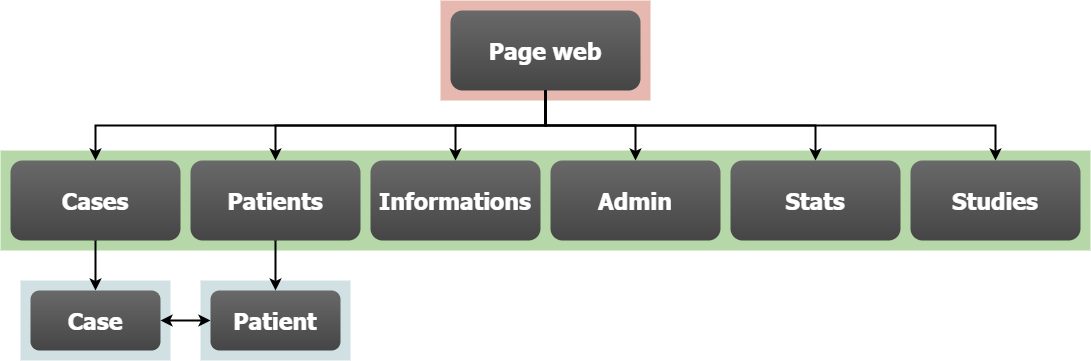
\includegraphics[width=1\textwidth]{images/conception/structure_navigation}
			\caption{La structure de la hiérarchie et navigation entre les vues}
			\label{structure_navigation}
		\end{figure}

	\subsection{Maquettes}

		Des maquettes de l'interface ont été réalisées dès le début du projet. Celles-ci ne sont typiquement pas totalement fidèles à ce que ressemblera la solution finale ; le but est de montrer la structure de la navigation, ainsi que se donner les moyens de les améliorer sur le temps et de s'assurer que l'on comprenne les features demandées. La figure~\ref{maquette_papier} montre par exemple la toute première ébauche de la page des cas, et la figure ~\ref{maquette_papier2} montre la même version de la vue d'un cas particulier.

		\begin{figure}[!h]
			\centering
			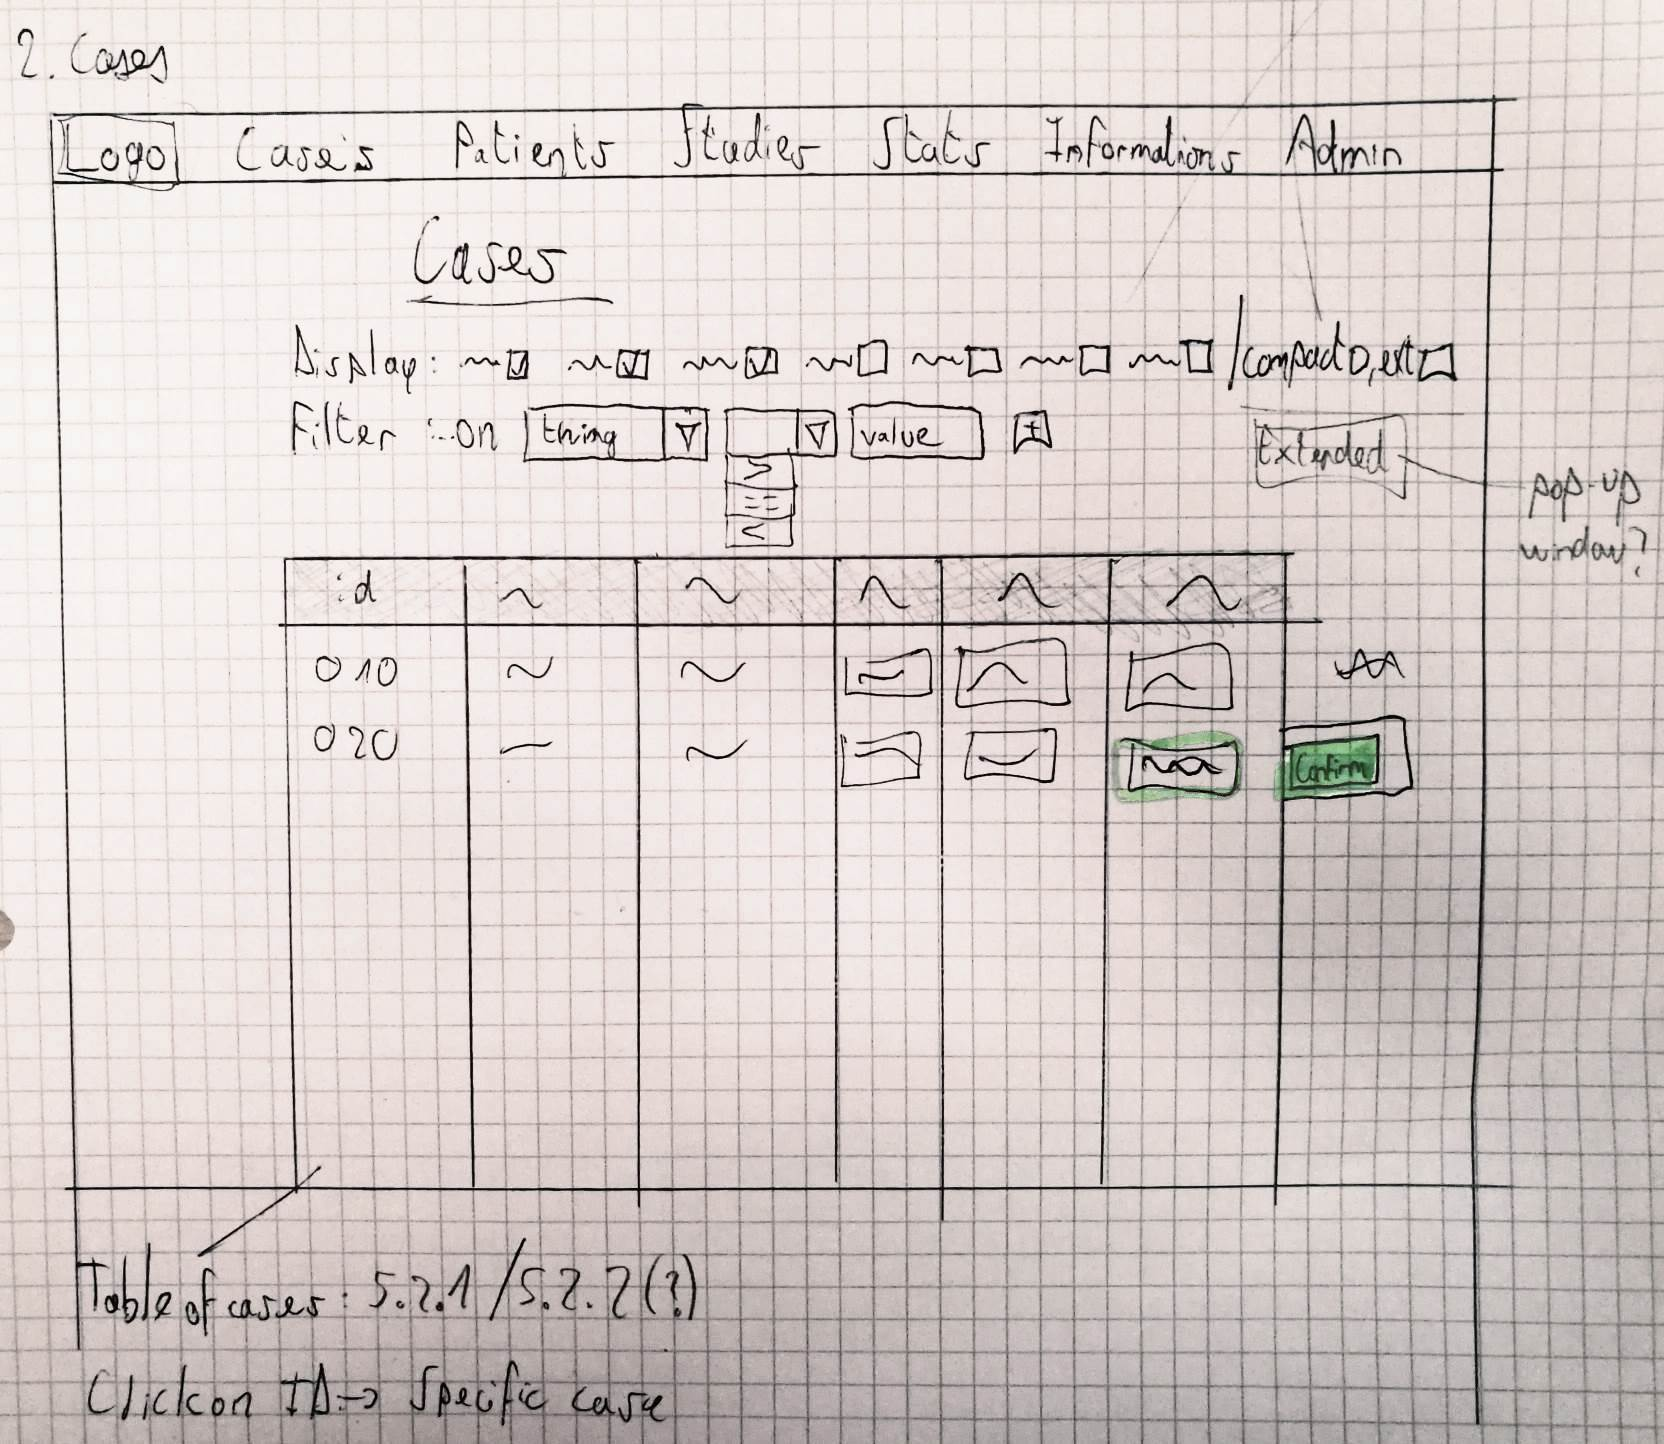
\includegraphics[width=1\textwidth]{images/analyse/maquette1}
			\caption{Wireframe sur papier de l'interface de la liste des cas}
			\label{maquette_papier}
		\end{figure}

		\begin{figure}[!h]
			\centering
			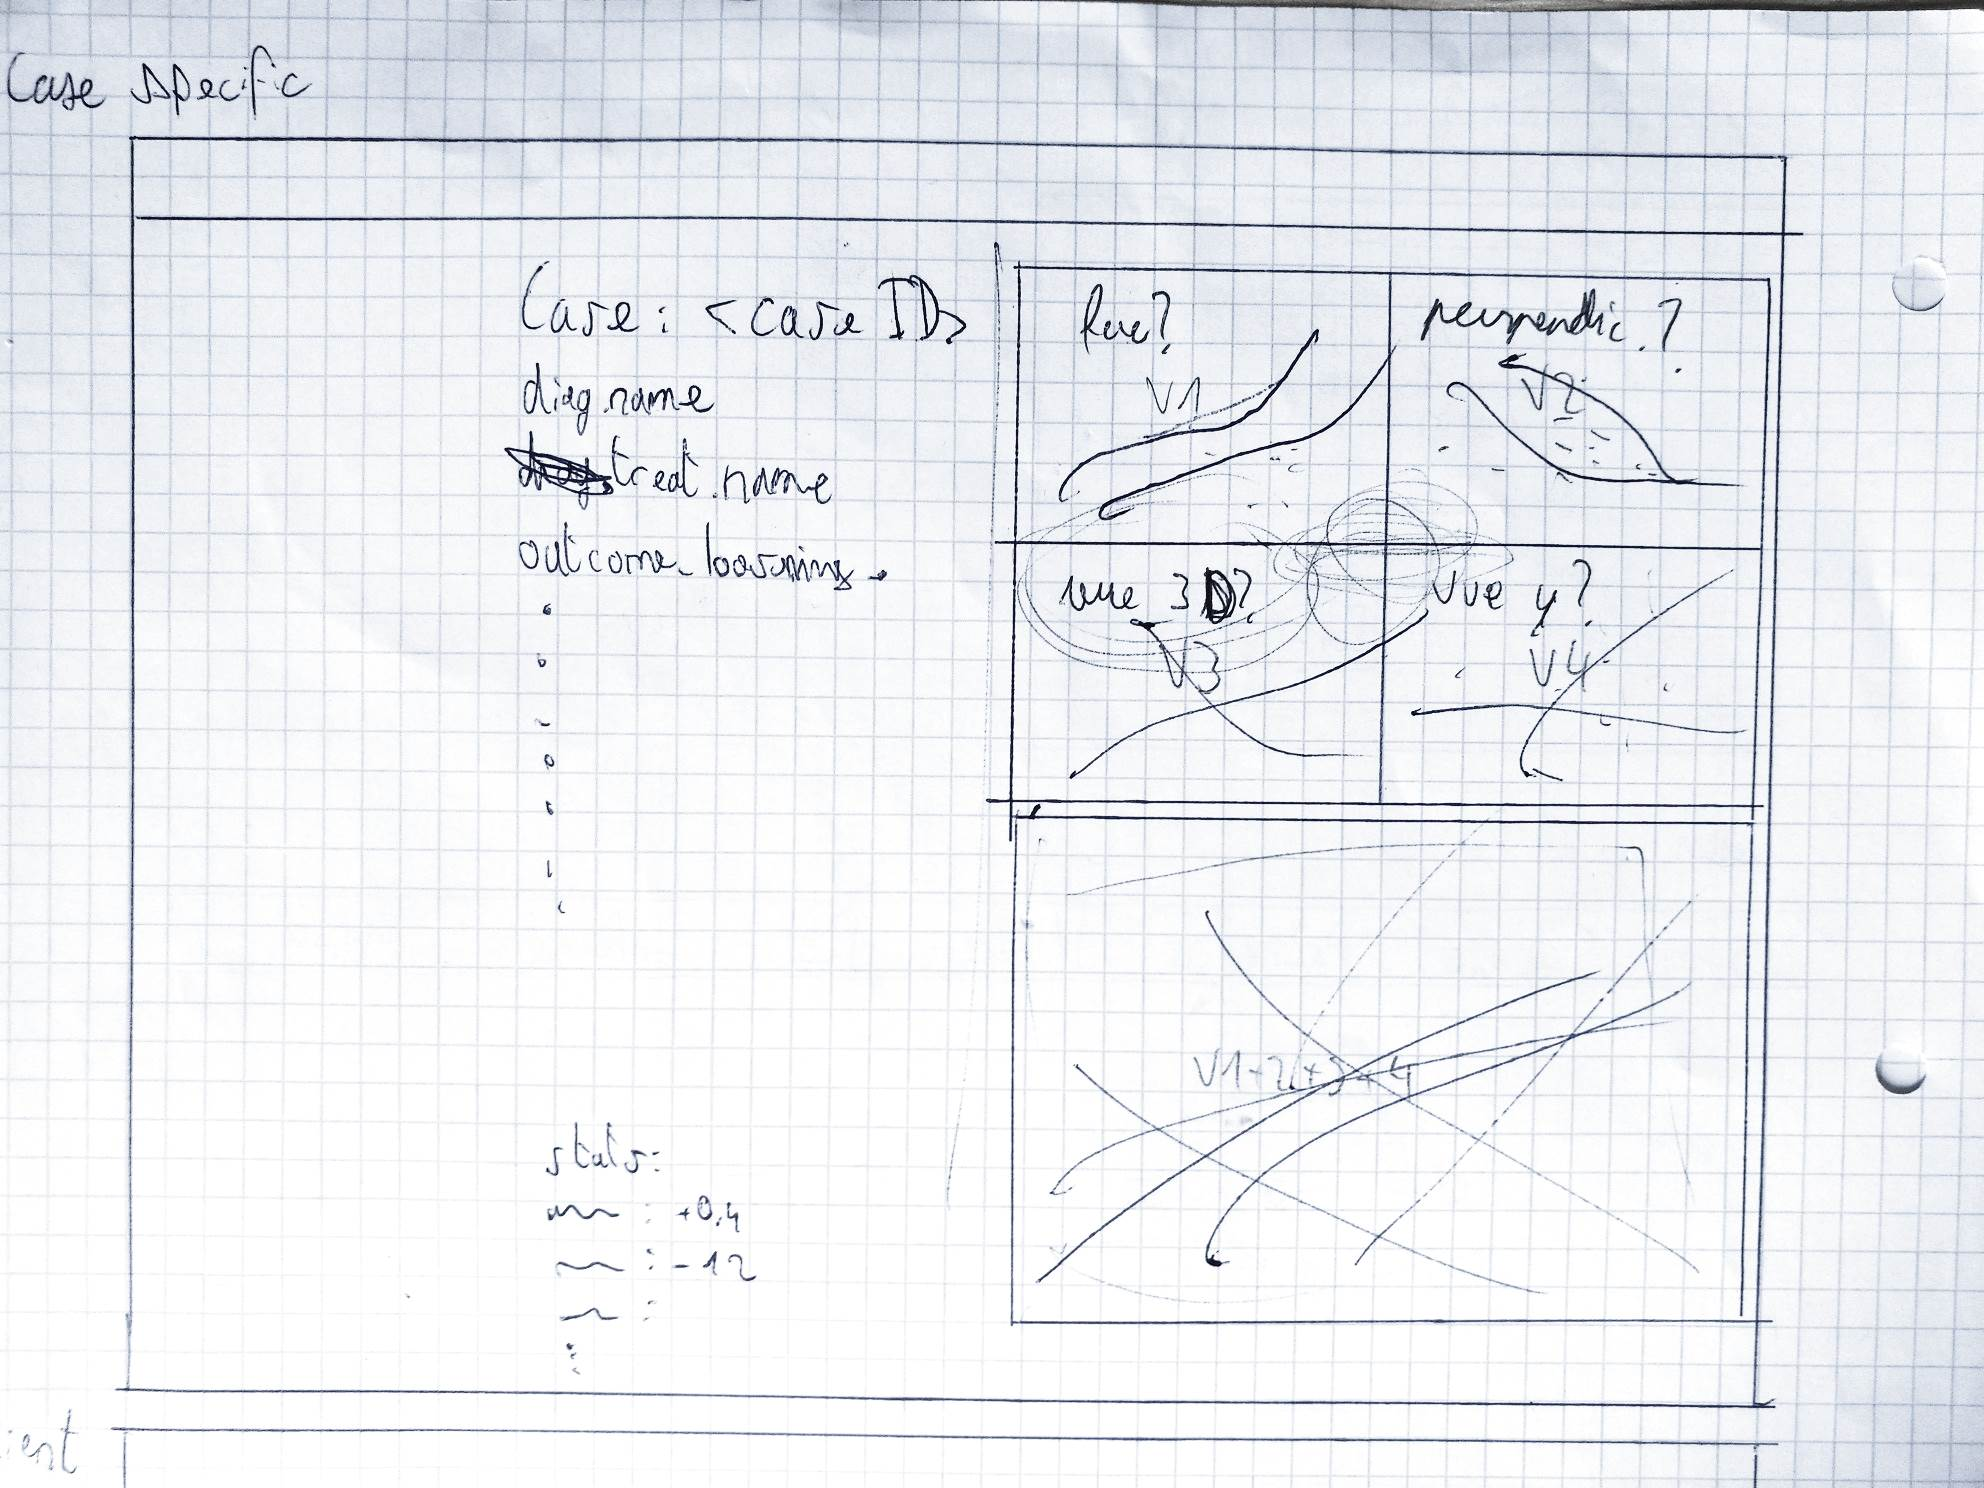
\includegraphics[width=1\textwidth]{images/analyse/maquette2}
			\caption{Maquette sur papier de l'interface d'un cas particulier}
			\label{maquette_papier2}
		\end{figure}

		La figure \ref{maquette_papier3} montre un sketch de deux pages secondaires au projet : une page d'administration ainsi qu'une page de statistiques.

		\begin{figure}[!h]
			\centering
			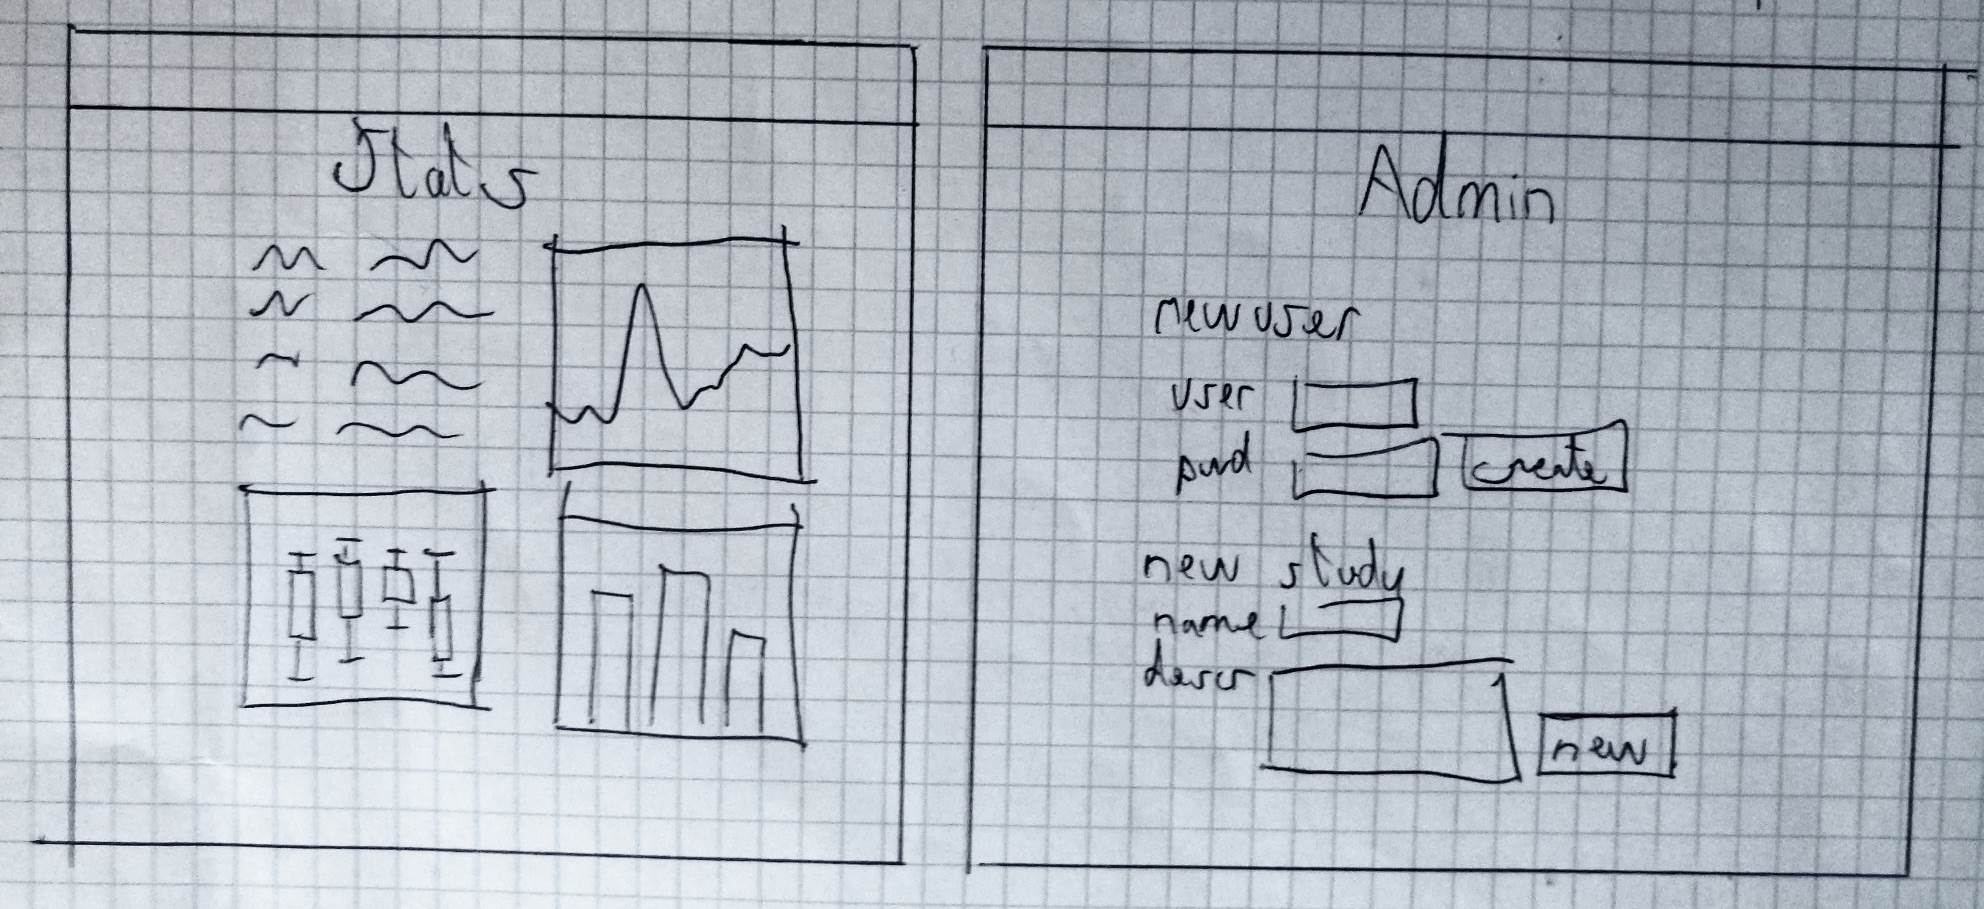
\includegraphics[width=1\textwidth]{images/analyse/maquette3}
			\caption{Sketch sur papier des pages "Stats" et "Admin"}
			\label{maquette_papier3}
		\end{figure}

\section{Implémentation frontend}

	L'implémentation du frontend a commencé par le choix et l'installation de l'environnement et des outils nécessaires pour développer en React de manière efficace. Le chapitre \ref{techno-react} explique l'utilité de chacun des composants, mais nous allons nous simplifier le travail en utilisant une configuration déjà prête pour le développement en React. Celle-ci est tirée du code annexe à la série de tutoriels suivis. Le code de cette configuration est disponible sur GitHub \cite{react-boilerplate}, et il s'agit de la configuration que j'ai utilisée. Tout le code décrit plus tard repose donc sur cette configuration.

	Le premier prototype s'est concentré sur l'implémentation des aspects qui ont été estimés comme étant centraux à l'application. Voici une liste des fonctionnalités du côté frontend qui doivent être implémentées pour réaliser le prototype :

	\begin{itemize}
		\item Disposition générale des éléments de la page
		\item Routage de chaque page sur sa vue correspondante
		\item Implémentation des pages "Patients" et "Cases"
		\item Lien avec les données de la base de données
	\end{itemize}

	\subsection{Disposition générale des éléments sur la page}

		Avant de démarrer à organiser les éléments d'une page, il est d'abord essentiel d'organiser les informations qui sont communes à toutes les pages. Comme le montre la figure \ref{maquette_papier}, il est prévu de naviguer entre les pages via une barre contenant les liens des autres vues, et qui se situe en haut de la page actuelle. 

		Toutefois, la décision a été prise de respecter au maximum les guidelines de Material Design\cite{material-design-guidelines}. Ici, il est préconisé d'utiliser une barre vertical contenant les liens vers les vues, appelée ``\texttt{Drawer}''. Ce Composant est d'ailleurs disponible dans la librairie Material-UI, mais il n'a pas pu être utilisé directement car il ne permet pas d'être continuellement visible. Dans ce cas ainsi que comme dans plusieurs cas dans le reste de l'application, il est nécessaire de l'implémenter en utilisant uniquement le CSS fourni par Material Design.

		Les liens vont donc rester sur la gauche de la page, et la vue principale sera affichée dans la partie droite.

		\begin{figure}[!ht]
			\centering
			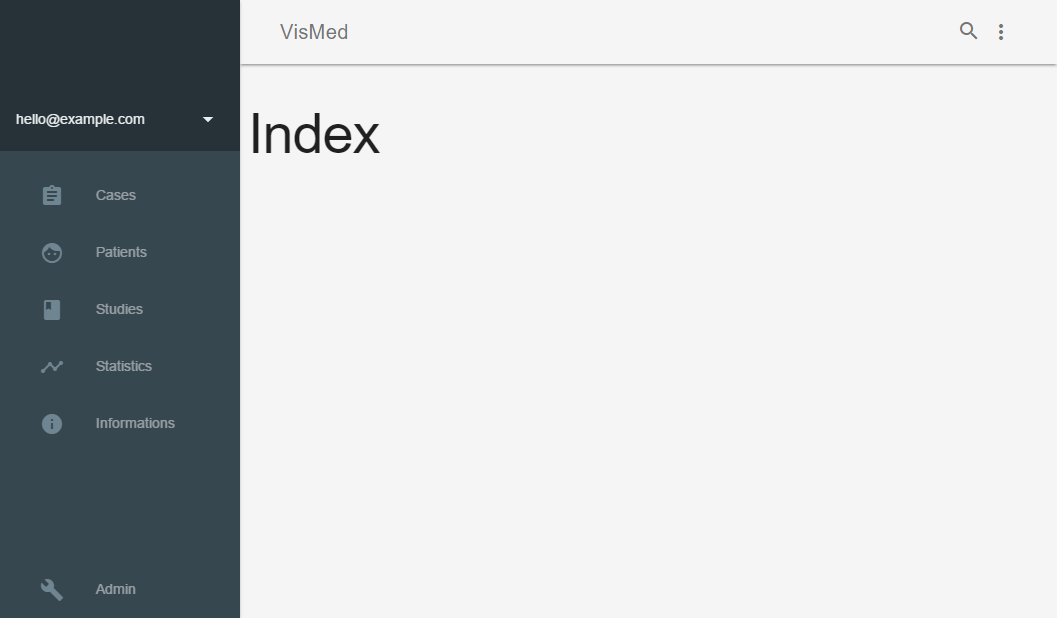
\includegraphics[width=1\textwidth]{images/realisation/proto1_1}
			\caption{Premier prototype fonctionnel de l'application}
			\label{proto1_1}
		\end{figure}

		La figure \ref{proto1_1} montre une des premières versions de la page, avec les liens du menu à gauche de celle-ci.

	\subsection{Routage}

		Etant donné que le but est de réaliser une "one-page app", nous allons utiliser une méthode de routage bien intégrée à React. Plutôt que télécharger une vue depuis le serveur à chaque fois que l'on désire changer de page, l'application entière est téléchargée au lancement de la page, et le changement de vue ainsi que le routage des liens se fait du côté client.

		Cet effet est accompli à l'aide de la librairie React-Router\cite{react-router}. Elle permet de déclarer quel Composant doit s'afficher en fonction de l'URL demandée, et de naviguer entre les vues sans rafraîchir la page complète.

\begin{figure}[!h]
\begin{lstlisting}[language=html]
<Router>
  <MuiThemeProvider muitheme={muiTheme}>
    <div class="mdl-layout_container">
      <div class="demo-layout mdl-layout mdl-js-layout mdl-layout--fixed-drawer mdl-layout--fixed-header">
        <Header/>
        <Aside/>
        <main class="mdl-layout__content mdl-color--grey-100">
          <div class="mdl-grid demo-content">
            <Route path="/" exact={true} name="index" component={Index}></Route>
            <Route path="/cases" name="cases" component={Cases}></Route>
            <Route path="/patients" name="patients" component={Patients}></Route>
            <Route path="/studies" name="studies" component={Studies}></Route>
            <Route path="/statistics" name="statistics" component={Statistics}></Route>
            <Route path="/informations" name="informations" component={Informations}></Route>
            <Route path="/admin" name="admin" component={Admin}></Route>
          </div>
        </main>
      </div>
    </div>
  </MuiThemeProvider>
</Router> \end{lstlisting}
\caption{Uutilisation des composants \texttt{Router} et \texttt{Route}}
\label{router-component}
\end{figure}

		La figure \ref{router-component} montre comment est déclaré le Router, ainsi que les différentes Routes de l'application. Le composant \texttt{Router} se trouve tout en haut de la hiérarchie, et c'est à l'intérieur de lui que les autres composants vont se placer. On peut voir qu'il n'y a aucun problème à mélanger du HTML (comme aux lignes 3 et 4) avec des composants React. Ce morceau de code représente à peu de choses près tout ce qui sera affiché sur les pages de l'application. Voici une liste des composants qu'on y trouve, et leur utilité :

		\begin{description}
			\item[\texttt{Router}] Englobe tous les composants devant pouvoir s'afficher ou se cacher selon l'URL demandée. Il doit donc englober toutes les \texttt{Route}s de l'application.
			\item[\texttt{MuiThemeProvider}] Nécessaire pour l'utilisation de la librairie Material-UI. Doit englober tous les éléments désirant utiliser des composants de cette librairie.
			\item[\texttt{Header}] Barre horizontale se trouvant au haut de la page. Affiche le titre de la page actuellement visitée.
			\item[\texttt{Aside}] Barre à gauche de la page, contenant les liens vers les différentes vues.
			\item[\texttt{Route}] Définit une route associée à une URL particulière, et quel composant afficher dans le cas où l'URL correspond à cette Route.
		\end{description}

		On voit donc ainsi que chaque Route va permettre d'afficher une page particulière. Par exemple, la ligne 10 traite le cas où l'URL se termine par \texttt{/cases}, et va donc se charger d'afficher le composant \texttt{Cases} à cet endroit. Chaque composant référencé par une \texttt{Route} (\texttt{Index}, \texttt{Cases}, \texttt{Patients}, \texttt{Studies} etc...) affiche donc sa vue lorsqu'il est appelé par le Router.

	\subsection{Pages "Patients" et "Cases"}

		Dans ce prototypes, les pages "Patients" et "Cases" sont très similaires. La figure montre la vue de la page "Patients".

		\begin{figure}[!ht]
			\centering
			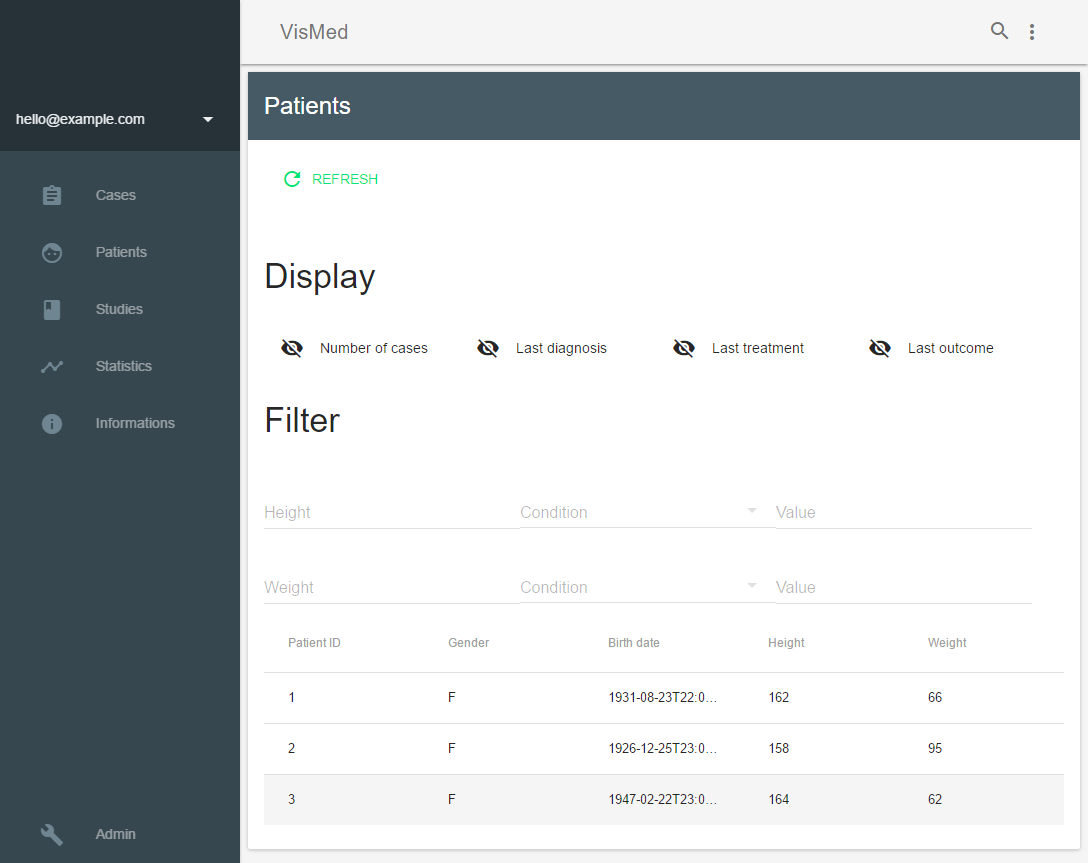
\includegraphics[width=1\textwidth]{images/realisation/proto1_2}
			\caption{Premier prototype de la page "Patients"}
			\label{proto1_2}
		\end{figure}

		On remarque que celle-ci reprend au mieux les éléments dessinés sur la maquette de la figure \ref{maquette_papier}. À nouveau, certains éléments ont été implémentés à l'aide de Material-UI, mais certains autres ont également dû être implémentés en utilisant directement le CSS de Material Design.

		Le principal élément de la page est un tableau présentant les données résumées de l'ensemble des patients. Ici, il s'agit de données d'exemple.

		Le but est ici de permettre deux actions différentes sur la liste des patients affichés : La partie "Display" permet d'afficher ou de cacher certaines colonnes, et la partie "Filter" permet. À noter que bien que l'interface soit implémentée ici, toutes les parties visibles ne sont pas encore fonctionnelles à ce stade. Les données affichées ne sont des données d'exemple, et les inputs de l'utilisateur (sur les parties Display et Filter) sont sans effet.

	\subsection{Communication des données}

		Une fois que le frontend est capable d'afficher des informations, il est encore nécessaire de le faire communiquer avec le serveur afin d'afficher les vraies données.

		\subsubsection{Flux de données}

			Comme nous utilisons et suivons le modèle Flux, il est nécessaire d'établir la logique du flux des données. Comme décrit dans le chapitre Analyse, Flux recommande l'utilisation d'un flux unidirectionnel des données.

			\begin{figure}[!ht]
				\centering
				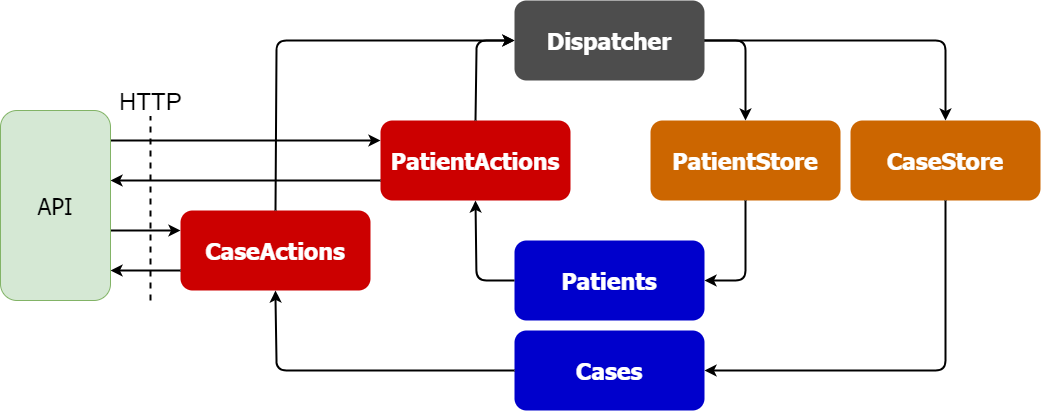
\includegraphics[width=1\textwidth]{images/realisation/vismedflux}
				\caption{Flux de données de l'application}
				\label{vismedflux}
			\end{figure}

			En suivant leurs recommandations, il a été possible d'établir le schéma illustré à la figure \ref{vismedflux}, montrant la manière dont les données sont échangées à travers de l'application React. On y voit les différents Classes et Composants qui interagissent dans l'échange de données :
			\begin{description}
				\item[\texttt{CaseActions} et \texttt{PatientActions}] Classes qui vont communiquer avec l'API du serveur lorsqu'on leur en fait la demande. Vont demander les données, et les transmettre au \texttt{Dispatcher} une fois reçues.
				\item[\texttt{Dispatcher}] Classe provenant de Flux, qui s'occupe de transmettre les données reçues aux Stores qui les stockent.
				\item[\texttt{PatientStore} et \texttt{CaseStore}]
				Classes qui stockent les données reçues depuis le \texttt{Dispatcher}. Elles servent à alimenter les vues \texttt{Patients} et \texttt{Cases} en données lorsqu'elles en ont besoin.
				\item[\texttt{Patients} et \texttt{Cases}] Composants React qui affichent respectivement la liste des patients, et la liste des cas. Chaque composant s'attache à son Store respectif, et affiche les données de celui-ci.
			\end{description}

			Au lancement de l'application, \texttt{PatientActions} et \texttt{CaseActions} agissent en demandant au serveur les données une première fois, ce qui va déclencher le reste de la boucle de réaction et ainsi pouvoir fournir des données aux composants \texttt{Patients} et \texttt{Cases} lorsque ceux-ci doivent être affichés.

\section{Implémentation backend}

	\subsection{Structure du backend}

		Pour la réalisation de la connexion entre la partie applicative métier et la partie base de données, il a été nécessaire de s'adapter à la structure hiérarchique des machines hébergeant l'application à l'EPFL. En effet, une contrainte est que le serveur hébergeant la base de données MySQL est accessible uniquement depuis l'intérieur du réseau.

		Bien que cela ne soit pas un problème pour l'application finale qui tournera sur un serveur de l'EPFL, cela complique la phase de développement durant laquelle il est nécessaire d'utiliser un autre serveur de l'EPFL comme proxy pour s'y connecter.

		\begin{figure}[h]
			\centering
			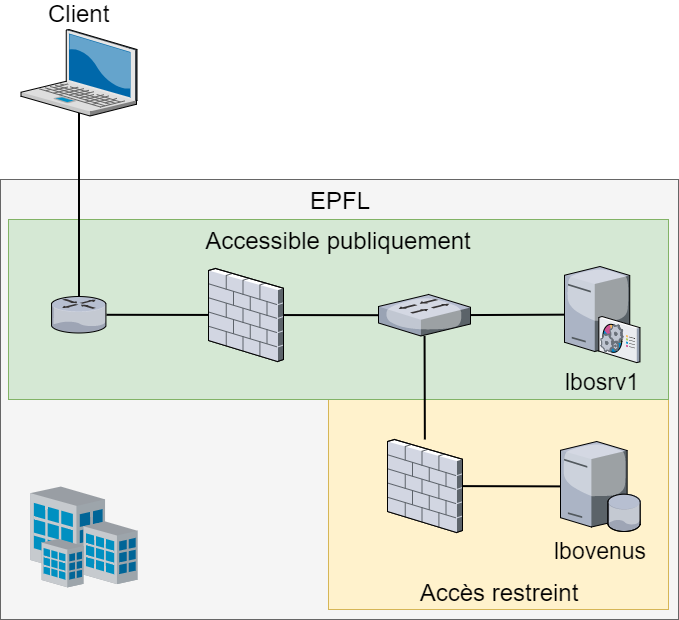
\includegraphics[width=1\textwidth]{images/realisation/Schema_EPFL}
			\caption{Schéma de l'architecture réseau de l'EPFL utilisée par VisMed}
			\label{schema-epfl}
		\end{figure}

		La figure~\ref{schema-epfl} montre, parmi l'architecture de l'EPFL traversée, les deux serveurs utilisés par l'installation de VisMed. On y voit :
		\begin{description}
			\item[lbosrv1] Il s'agit du serveur "principal", sur lequel tourne le code backend de l'application. Il s'agit également du serveur qui va écouter le port 80, et donc recevoir les requêtes HTTP de clients externes et y répondre. Mais afin de pouvoir faire son travail correctement, il aura généralement besoin d'accéder à des données se trouvant sur la base de données des cas et des patients. Celle-ci se trouve sur le deuxième serveur utilisé, qui se nomme \texttt{lbovenus}.
			\item[lbovenus] Il s'agit du serveur contenant la base de données médicales actuelle. Celle-ci, de type MySQL, contient les données concernant les patients de l'hôpital, ainsi que leurs cas. Cette base de données se trouve derrière un pare-feu supplémentaire, et est inaccessible depuis l'extérieur de l'EPFL. Le seul moyen de pouvoir la questionner est d'être à l'intérieur du réseau de l'EPFL, où se trouve également \texttt{lbosrv1}. C'est pourquoi il y a accès sans problème.
		\end{description}

	\subsection{Express.js}

		La logique du serveur a été développée en utilisant node.js ainsi que la librairie Express. Express s'occupe d'écouter sur un port particulier et de répondre aux requêtes avec les informations adéquates. Dans notre cas, le port utilisé est le \texttt{3000}. Elle sert les quelques ressources statiques nécessaires (script JavaScript dont l'application compilée, mais également les fichiers CSS). Mais également, elle répond aux requêtes sur l'API définie.

		Les requêtes possibles de l'API sont peu nombreuses :

		\begin{description}
			\item[\texttt{GET /api/patients}] Renvoie la liste complète des patients ainsi que toutes leurs informations.
			\item[\texttt{GET /api/cases}] Renvoie la liste complète des patients ainsi que toutes leurs informations.
		\end{description}

		Pour fournir les informations nécessaires lors de l'appel à l'un de ces deux méthodes, l'application se connecte à la base de données, effectue une requête sur la vue correspondante, et formate le résultat pour l'envoyer en JSON au client.

	\subsection{Base de données}

		Pour simplifier la sélection des données utiles à partir de la structure initiale de la base de données, des vues SQL ont été ajoutées.
		Les deux vues, \texttt{case\_view\_all} et \texttt{patient\_view\_all}, joignent toutes les données nécessaires de plusieurs tables afin de constituer la réponse voulue aux requêtes sur les deux méthodes de l'API précédemment décrites.

\section{Evaluation}

	\subsection{Heuristique et adaptations}

		Ce prototype a été discuté à de nombreuses reprises.
		Des évaluations ont été faites de semaine en semaine, et ont mené à de nombreuses améliorations basées sur des critères ergonomiques.

		Durant ces séances d'évaluation heuristique, beaucoup de points discutés ont été à adapter afin de proposer une interface avec une meilleure ergonomie. Les modifications qui en résultent suivent les critères ergonomiques de Bastien et Scapin\cite{ergoweb} tels que la cohérence, la lisibilité ou le principe du groupement/distinction. Par exemple, sur la page Patients, on peut noter :

		\begin{itemize}
			\item Augmentation de la taille de police
			\item Retrait des titres "Display" et "Filter"
			\item Elargissement de la zone d'affichage à toute la largeur de la page
			\item Utilisation du Header pour y placer les filtres de display
			\item Retrait du bouton d'actualisation
			\item Augmentation de la visibilité des titres de colonne
		\end{itemize}

		De même, des changements plus généraux ont été appliqués :

		\begin{itemize}
			\item Augmentation de la taille de police des liens
			\item Augmentation du contraste de la police et des icônes des liens
			\item Retrait du titre "VisMed" dans le Header
			\item Passage du bouton "Admin" en haut du Drawer, avec les autres liens
			\item Surbrillance du lien actuellement sélectionné
		\end{itemize}

		Les évaluations heuristiques ont donc permis au prototype d'évoluer à la fois en termes de fonctionnalités grâce au contact avec le client, et à la fois utilisabilité grâce aux critères d'ergonomie qui ont été appliqués. Les adaptations se sont fait itérativement sur plusieurs semaines, et ont mené à la production d'un deuxième prototype. 

	\subsection{Validation par les clients}

		Les prototypes ont été montrés au client à plusieurs reprises afin de bénéficier d'un feedback, en plus de la première réunion en personne avec tous les intervenants. La confirmation de celui-ci de la direction du développement nous a permis de s'assurer que le projet allait dans le sens demandé.